%----------------------------------------------------------------------------------------
%    PACKAGES AND THEMES
%----------------------------------------------------------------------------------------

\documentclass[aspectratio=169,xcolor=dvipsnames]{beamer}
\usetheme{SimpleDarkBlue}
\usepackage{colortbl}
\usepackage{hyperref}
\usepackage{graphicx}
\usepackage{booktabs}
\usepackage{amsmath}
\usepackage{amssymb}

\usepackage{multicol}
\usepackage{tikz}
\usetikzlibrary{shapes, arrows, positioning, calc}
\usepackage{animate}
\usepackage{array}

%----------------------------------------------------------------------------------------
%    TITLE PAGE
%----------------------------------------------------------------------------------------

\title[Understanding CNNs with CAPE Data]{Comprendre les Réseaux de Neurones Convolutifs\\ Application à l'Analyse des Données Météorologiques CAPE}


\author[M. El Abdioui \& A. Msaadi]{Mohammed El Abdioui \& Abdellah Msaadi}

\institute
{
    Projet de Machine Learning  \\
    Analyse des CNN à travers les Données Météorologiques
}
\date{\today}

%----------------------------------------------------------------------------------------
%    PRESENTATION SLIDES
%----------------------------------------------------------------------------------------

\begin{document}

\begin{frame}
    \titlepage
\end{frame}

%------------------------------------------------
\section{Introduction et Contexte}
%------------------------------------------------

\begin{frame}{Objectifs de cette Présentation}
    \begin{block}{Objectif Principal}
        Comprendre le fonctionnement et l'implémentation des Réseaux de Neurones Convolutifs (CNN) à travers un cas pratique réel
    \end{block}
    
    \begin{columns}[T]
        \column{0.5\textwidth}
        \textbf{Pourquoi ce projet?}
        \begin{itemize}
            \item Étude approfondie des CNN 1D
            \item Application à des données réelles complexes
            \item Comparaison des approches ML traditionnelles
            \item Analyse de performance détaillée
        \end{itemize}
        
        \column{0.5\textwidth}
        \textbf{Ce que nous allons couvrir}
        \begin{enumerate}
            \item Fondements théoriques des CNN
            \item Architecture détaillée
            \item Préparation des données
            \item Entraînement et optimisation
            \item Résultats et analyse
            \item Leçons apprises
        \end{enumerate}
    \end{columns}
    
    
\end{frame}

\begin{frame}{Pourquoi les CNN pour les Données Séquentielles?}
    \begin{figure}
        \centering
        \includegraphics[width=0.5\textwidth]{1-4.png}
        \caption{Notre architecture CNN 1D pour l'analyse des séries temporelles météorologiques}
    \end{figure}
    
    \begin{columns}[T]
        \column{0.33\textwidth}
        \textbf{RNN/LSTM}
        \begin{itemize}
            \scriptsize
            \item Mémoire temporelle
            \item Complexe à entraîner
            \item Problèmes de gradient
            \item Lent pour longues séquences
        \end{itemize}
        
        \column{0.33\textwidth}
        \textbf{CNN 1D}
        \begin{itemize}
            \scriptsize
            \item Extraction locale de motifs
            \item Entraînement parallèle
            \item Gradients stables
            \item Rapide et efficace
        \end{itemize}
        
        \column{0.33\textwidth}
        \textbf{Transformers}
        \begin{itemize}
            \scriptsize
            \item Attention globale
            \item Beaucoup de paramètres
            \item Besoin de beaucoup de données
            \item Coûteux en calcul
        \end{itemize}
    \end{columns}
    
  
\end{frame}

%------------------------------------------------
\section{Les Fondements des CNN}
%------------------------------------------------

\begin{frame}{L'Opération de Convolution: Base Mathématique}
    % Utilisation de \small pour compacter le contenu de la colonne de gauche
    \small 
    \begin{columns}[T]
        \column{0.55\textwidth} 
        \textbf{Définition Mathématique (Corrélation Croisée)}
        

        
        % Formule de la corrélation croisée 1D:
        \textbf{Corrélation Croisée 1D (en DL):}
        % Utilisation de \dfrac pour que l'équation soit mieux rendue en mode \small si besoin
        \[
        y[i] = \sum_{k=0}^{K-1} x[i + k] \cdot w[k] 
        \]
        
     
        
        \textbf{Dans une Couche de Réseau Neurale:}
        \[
        y_i = \sigma\left(\sum_{k=0}^{K-1} x_{i+k} \cdot w_k + b\right)
        \]
        \vspace{-0.55cm}
        \begin{block}{Paramètres Clés}
            \begin{itemize}
                \item $K$: Taille du noyau (kernel size)
                \item $w_k$: Poids appris
                \item $b$: Biais (bias)
                \item $\sigma$: Fonction d'activation (ex: ReLU)
            \end{itemize}
        \end{block}
        
        \column{0.5\textwidth}
        \textbf{Visualisation 1D (K=2)}
        \begin{figure}
            \centering
            % Réduction de l'échelle à 0.8 pour gagner de la place
            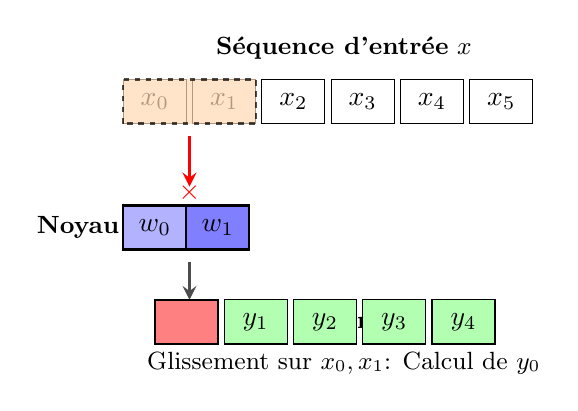
\begin{tikzpicture}[scale=0.8, >=stealth] 
                % 1. Séquence d'entrée X
                \node at (3.5, 5.2) {\small \textbf{Séquence d'entrée} $x$};
                \foreach \i in {0,...,5} {
                    \draw (\i*1.1, 4) rectangle (\i*1.1+1.0, 4.7);
                    \node at (\i*1.1+0.5, 4.35) {$x_{\i}$};
                }
                
                % 2. Noyau W
                \node at (-0.5, 2.35) {\small \textbf{Noyau} $w$};
                \draw[fill=blue!30, thick] (0, 2) rectangle (1.0, 2.7);
                \draw[fill=blue!50, thick] (1.0, 2) rectangle (2.0, 2.7);
                \node at (0.5, 2.35) {$w_0$};
                \node at (1.5, 2.35) {$w_1$};
                
                % 3. Position i=0 (Calcul de y_0)
                \only{\node at (3.5, 0.2) {\small Glissement sur $x_0, x_1$: Calcul de $y_0$ };}
                
                % Mise en évidence de l'entrée (i=0, i+1=1)
                \draw[fill=orange!30, opacity=0.7, thick, dash pattern=on 2pt off 2pt] (0, 4) rectangle (2.1, 4.7);
                
                % Flèche montrant l'opération
                \draw[->, very thick, red] (1.05, 3.8) -- (1.05, 3.0);
                \node[red] at (1.05, 2.9) {$\times$};
                
                % Flèche vers la sortie y_0
                \draw[->, very thick, black!70] (1.05, 1.8) -- (1.05, 1.2);
                
                % 4. Sortie Y
                \node at (4.0, 0.85) {\small \textbf{Sortie} $y$};
                \foreach \i in {0,...,4} {
                    \draw[fill=green!30] (\i*1.1+0.5, 0.5) rectangle (\i*1.1+1.5, 1.2);
                    \node at (\i*1.1+1.0, 0.85) {$y_{\i}$};
                }
                % Mise en évidence de la sortie y_0
                \draw[fill=red!50, thick] (0.5, 0.5) rectangle (1.5, 1.2);
                
            \end{tikzpicture}
        \end{figure}
        
        \vspace{-5pt}
        
        
        \textbf{Exemples pour $y_i$:}
        \[
        y_0 = \sigma(x_0 w_0 + x_1 w_1 + b)
        \]
        \[
        y_1 = \sigma(x_1 w_0 + x_2 w_1 + b)
        \]
    \end{columns}
\end{frame}

\begin{frame}{Propriétés Clés des CNN}
    \begin{columns}[T]
        \column{0.5\textwidth}
        \textbf{Connectivité Locale}
        \begin{itemize}
            \item Chaque neurone connecte à une région locale
            \item Réduction du nombre de paramètres
            \item Capture de motifs locaux
            
            \vspace{10pt}
            \textbf{Avantages:}
            \begin{itemize}
                \item Moins de paramètres
                \item Meilleure généralisation
                \item Extraction hiérarchique
            \end{itemize}
        \end{itemize}
        
        \begin{block}{Exemple avec nos données}
            \begin{itemize}
                \item Entrée: 12 features météo
                \item Noyau K=2: capture paires de features
                \item Combinaisons locales apprises
            \end{itemize}
        \end{block}
        
        \column{0.5\textwidth}
        \textbf{Partage des Poids (Weight Sharing)}
        \begin{itemize}
            \item Même filtre appliqué partout
            \item Invariance translationnelle
            \item Détection de motifs indépendante de la position
      
            \textbf{Équation:}
            \vspace{-0.3cm}
            \[
            \text{Même } w_k \text{ pour tout } i
            \]
              \vspace{-0.4cm}
            \[
            y_i = \sigma\left(\sum_{k} x_{i+k} \cdot w_k + b\right)
            \]
        \end{itemize}
          \vspace{-0.5cm}
        \begin{alertblock}{Bénéfices}
            \begin{itemize}
                \item Réduction radicale des paramètres
                \item Apprentissage de motifs génériques
                \item Robustesse aux translations
            \end{itemize}
        \end{alertblock}
    \end{columns}
\end{frame}

\begin{frame}{Fonctions d'Activation et Propagation}
    \footnotesize % Taille de police globale réduite pour tout faire tenir
    
    \begin{columns}[T, onlytextwidth]
        \column{0.48\textwidth}
        \textbf{ReLU (Rectified Linear Unit)}
        \begin{equation*}
            \text{ReLU}(x) = \max(0, x)
        \end{equation*}
        
        \begin{itemize}
            \item Simplicité computationnelle
            \item Pas de gradient vanishing
            \item Convergence plus rapide
        \end{itemize}
        
        \textbf{Dans notre modèle :}
        \begin{itemize}
            \item Après chaque couche Conv1D
            \item Introduction de non-linéarité
        \end{itemize}
        
        \begin{figure}
            \centering
            \begin{tikzpicture}[scale=0.5] % Échelle réduite de 0.6 à 0.5
                \draw[->] (-2,0) -- (2,0) node[right] {\tiny $x$};
                \draw[->] (0,-0.5) -- (0,1.8) node[above] {\tiny ReLU};
                \draw[thick, blue] (-2,0) -- (0,0) -- (1.5,1.5);
                \node[blue] at (0.8,1.2) ;
            \end{tikzpicture}
        \end{figure}
        
        \column{0.48\textwidth}
        \textbf{Propagation Avant / Arrière}
        
        \textit{Forward :}
        \begin{align*}
            z^{(l)} &= W^{(l)} a^{(l-1)} + b^{(l)} \\
            a^{(l)} &= \sigma(z^{(l)})
        \end{align*}
        
        \vspace{-10pt} % Gain de place vertical
        
        \textit{Backward :}
        \begin{align*}
            \delta^{(l)} &= \partial \mathcal{L} / \partial z^{(l)} \\
            \partial \mathcal{L} / \partial W^{(l)} &= \delta^{(l)} (a^{(l-1)})^T \\
            \partial \mathcal{L} / \partial b^{(l)} &= \delta^{(l)}
        \end{align*}
        
        \vspace{-5pt}
        
        \begin{block}{Chaîne de Convolution}
            \begin{itemize}[leftmargin=*] % Marges réduites
                \item Matrice \textbf{Toeplitz} pour l'efficacité
                \item Implémentation via \textbf{im2col}
            \end{itemize}
        \end{block}
    \end{columns}
\end{frame}

%------------------------------------------------
\section{Architecture Détaillée de Notre Modèle}
%------------------------------------------------

\begin{frame}{Architecture Complète: Vue d'Ensemble}
    \begin{figure}
        \centering
        \includegraphics[width=0.5\textwidth]{1-4.png}
        \caption{Architecture détaillée de notre CNN 1D avec toutes les couches et connexions}
    \end{figure}
    
    \begin{columns}[T]
        \column{0.33\textwidth}
        \textbf{Bloc d'Entrée}
        \begin{itemize}
            \footnotesize
            \item Shape: (batch, 1, 12)
            \item 12 variables météo
            \item Normalisation batch
            \item Ajustement dimensionnel
        \end{itemize}
        
        \column{0.33\textwidth}
        \textbf{Blocs Convolutifs}
        \begin{itemize}
            \footnotesize
            \item 2 couches Conv1D
            \item Filtres: 64 → 128
            \item Kernel size: 2
            \item Padding: 'same'
        \end{itemize}
        
        \column{0.33\textwidth}
        \textbf{Couches Denses}
        \begin{itemize}
            \footnotesize
            \item 128 → 64 neurones
            \item Dropout: 0.3, 0.15
            \item Régularisation L2
            \item Sortie: 1 valeur
        \end{itemize}
    \end{columns}
    

\end{frame}

\begin{frame}{Couche par Couche: Paramètres et Dimensions}
    \begin{table}
        \tiny
        \begin{tabular}{p{2.5cm}p{1.5cm}p{1.5cm}p{1.2cm}p{3cm}}
            \toprule
            \textbf{Couche} & \textbf{Shape Sortie} & \textbf{Paramètres} & \textbf{Activation} & \textbf{Opérations Spéciales} \\
            \midrule
            InputLayer & (1, 12) & 0 & - & Reshape pour Conv1D \\
            \rowcolor{blue!10}
            Conv1D-1 & (1, 64) & 1,600 & ReLU & K=2, padding='same', L2(0.001) \\
            BatchNorm-1 & (1, 64) & 256 & - & $\gamma, \beta$ pour 64 canaux \\
            Dropout-1 & (1, 64) & 0 & - & Rate=0.15 pendant training \\
            \rowcolor{blue!10}
            Conv1D-2 & (1, 128) & 16,512 & ReLU & K=2, padding='same', L2(0.001) \\
            BatchNorm-2 & (1, 128) & 512 & - & Normalisation par batch \\
            \rowcolor{green!10}
            GlobalAvgPool1D & (128) & 0 & - & $y_c = \frac{1}{T}\sum_t x_{t,c}$ \\
            \rowcolor{orange!10}
            Dense-1 & (128) & 16,512 & ReLU & Fully connected, L2(0.001) \\
            BatchNorm-3 & (128) & 512 & - & Normalisation après dense \\
            Dropout-2 & (128) & 0 & - & Rate=0.30 (forte régularisation) \\
            \rowcolor{orange!10}
            Dense-2 & (64) & 8,256 & ReLU & Réduction dimension, L2(0.001) \\
            BatchNorm-4 & (64) & 256 & - & Dernière normalisation \\
            Dropout-3 & (64) & 0 & - & Rate=0.15 \\
            \rowcolor{red!10}
            Output (Dense) & (1) & 65 & Linear & Sortie finale, pas d'activation \\
            \midrule
            \textbf{Total} & & 44,481 & & \\
            \textbf{Trainable} & & 43,713 & & 98.3\% des paramètres \\
            \textbf{Non-trainable} & & 768 & & BatchNorm $\gamma,\beta$ \\
            \bottomrule
        \end{tabular}
    \end{table}
    
   \begin{block}{Analyse de l'Architecture}
    \vspace{-10pt} % Ajout pour remonter le contenu du bloc
    \begin{columns}[T]
        \column{0.5\textwidth} % Colonne de gauche (50% de la largeur du bloc)
        % Réduction de l'espace vertical et horizontal
        \begin{itemize} 
            \setlength{\itemsep}{0pt} % Supprime l'espace vertical entre les items
            \setlength{\leftmargin}{0pt} % Tente de réduire la marge (moins efficace que itemsep)
            \scriptsize
            \item \textbf{Profondeur}: 13 couches fonctionnelles
            \item \textbf{Largeur}: 64$\rightarrow$128 filtres, 128$\rightarrow$64 neurones denses
        \end{itemize}

        \column{0.5\textwidth} % Colonne de droite (50% de la largeur du bloc)
        % Réduction de l'espace vertical et horizontal
        \begin{itemize} 
            \setlength{\itemsep}{0pt} % Supprime l'espace vertical entre les items
            \setlength{\leftmargin}{0pt} % Tente de réduire la marge
            \scriptsize
            \item \textbf{Efficacité}: 44K paramètres seulement
            \item \textbf{Régularisation}: 5 mécanismes différents
        \end{itemize}
    \end{columns}
\end{block}
\end{frame}

\begin{frame}{Régularisation: Combattre le Sur-Apprentissage}
    \footnotesize % Police générale légèrement réduite

    % --- Structure du haut (Contenu Technique) ---
    \begin{columns}[T]
        % Col 1 (28%): Dropout
\column{0.28\textwidth}
\textbf{Dropout}
\[
\tilde{x}_i = 
\begin{cases}
    \frac{x_i}{1-p} & \text{si prob. } 1-p \\ % CORRECTION (Utilise "si prob." pour la clarté)
    0 & \text{si prob. } p
\end{cases}
\]
        \vspace{-5pt}
        \begin{itemize} 
            \setlength{\itemsep}{0pt} 
            \tiny
            \item \textbf{Rates}: 0.15 (conv), 0.30 (dense1), 0.15 (dense2)
            \item \textbf{Effet}: Empêche la co-adaptation
        \end{itemize}
        
        % Col 2 (28%): Batch Normalization
        \column{0.28\textwidth}
        \textbf{Batch Normalization}
        \[
        \hat{x} = \frac{x - \mu_B}{\sqrt{\sigma_B^2 + \epsilon}}
        \]
        \[
        y = \gamma \hat{x} + \beta
        \]
        \vspace{-5pt}
        \begin{itemize} 
            \setlength{\itemsep}{0pt}
            \tiny
            \item \textbf{Paramètres}: $\gamma, \beta$ appris
            \item \textbf{Avantages}: Stabilisation, LR plus élevé
        \end{itemize}
        
        % Col 3 (22%): L2 Regularization
        \column{0.22\textwidth}
        \textbf{L2 Regularization}
        \[
        \mathcal{L}_{\text{total}} = \mathcal{L}_{\text{data}} + \lambda \sum w_i^2
        \]
        \vspace{-5pt}
        \begin{itemize} 
            \setlength{\itemsep}{0pt}
            \tiny
            \item \textbf{$\lambda$}: 0.001
            \item \textbf{Effet}: Pénélisation des grands poids
        \end{itemize}
        
        % Col 4 (22%): Early Stopping
        \column{0.22\textwidth}
        \textbf{Early Stopping}
        \begin{itemize} 
            \setlength{\itemsep}{0pt}
            \tiny
            \item \textbf{Monitor}: Val. loss
            \item \textbf{Patience}: 15 epochs
            \item \textbf{Modèle}: Restauré
        \end{itemize}
    \end{columns}
    
    \vspace{1cm} % Réduire l'espace vertical
    
    % --- Structure du bas (Synthèse et Figure) ---
    \begin{columns}[T]
        % Col 5 (Gauche): Synthèse et Explication
        \column{0.5\textwidth}
        \vspace{-10pt} % Remonter le contenu pour compenser
        \begin{block}{Synthèse et Stratégie}
            \textbf{\small Combinaison de 4 méthodes : Forte robustesse.}
        \end{block}
        \vspace{-5pt}
        \begin{itemize}
            \tiny
            \item Objectif : Maximiser la \textbf{généralisation} des prédictions.
            \item L'efficacité repose sur l'équilibre de ces techniques.
        \end{itemize}
        
        % Col 6 (Droite): Figure (En bas à droite)
        \column{0.5\textwidth}
        \begin{figure}
            \centering
            % Figure TikZ compactée
            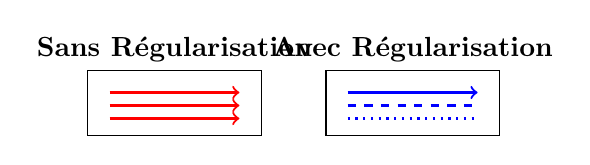
\begin{tikzpicture}[scale=0.55] % Échelle encore légèrement réduite pour l'espace
                % Sans régularisation
                \draw (0,0) rectangle (4,1.5);
                \node at (2,2) {\textbf{Sans Régularisation}};
                \draw[red, thick, ->] (0.5,1) -- (3.5,1);
                \draw[red, thick, ->] (0.5,0.7) -- (3.5,0.7);
                \draw[red, thick, ->] (0.5,0.4) -- (3.5,0.4);
                
                % Avec régularisation
                \draw (5.5,0) rectangle (9.5,1.5);
                \node at (7.5,2) {\textbf{Avec Régularisation}};
                \draw[blue, thick, ->] (6.0,1) -- (9.0,1);
                \draw[blue, thick, dashed] (6.0,0.7) -- (9.0,0.7);
                \draw[blue, thick, dotted] (6.0,0.4) -- (9.0,0.4);
            \end{tikzpicture}
            \vspace{-10pt}
            \caption{\tiny L'effet de la régularisation sur les chemins d'activation.}
        \end{figure}
    \end{columns}
\end{frame}

%------------------------------------------------
\section{Préparation et Analyse des Données}
%------------------------------------------------

\begin{frame}{Données Météorologiques: Vue d'Ensemble}
    \footnotesize % Taille de police de base

    \begin{columns}[T]
        % --- Colonne 1 (45%): Figure ---
        \column{0.45\textwidth}
        \begin{figure}
            \centering
            % Réduction de la taille de l'image
            \includegraphics[width=\columnwidth]{CApe.png} 
            \vspace{-5pt} % Réduire l'espace sous la légende
            \caption{\tiny Distribution spatiale des points d'échantillonnage à travers le Maroc.}
            \label{fig:spatial_distribution}
        \end{figure}
        
        \column{0.55\textwidth}
        % --- Colonne 2 (55%): Texte et Stratégies ---
        
        \textbf{Caractéristiques du Dataset}
        \begin{itemize} % RETRAIT DES OPTIONS NON SUPPORTÉES
            \setlength{\itemsep}{0pt} % COMPACTAGE VERTICAL STANDARD
            \tiny
            \item \textbf{Source}: Réanalyse météorologique 2024
            \item \textbf{Format}: NetCDF
            \item \textbf{Résolution}: $1$ heure $\times$ $0.5^{\circ}$ $\times$ $0.5^{\circ}$
            \item \textbf{Couverture}: 20$^{\circ}$N-40$^{\circ}$N, 20$^{\circ}$W-5$^{\circ}$E
        \end{itemize}
        
        \vspace{-5pt}
        
        \textbf{Stratégie d'Échantillonnage}
        \begin{itemize} % RETRAIT DES OPTIONS NON SUPPORTÉES
            \setlength{\itemsep}{0pt} % COMPACTAGE VERTICAL STANDARD
            \tiny
            \item \textbf{Temporel}: 10\% aléatoire (878/8784 heures)
            \item \textbf{Spatial}: 1 point sur 2 (41$\times$51 vs 81$\times$101)
            \item \textbf{Final}: 1.8M échantillons (2.55\% original)
            \item \textbf{CIN}: Imputation des 95\% NaN par 0
        \end{itemize}
        
        \vspace{-5pt}
        
        \begin{alertblock}{Défi Principal}
            \tiny
            71 millions d'échantillons originaux $\rightarrow$ nécessité d'échantillonnage intelligent
        \end{alertblock}
        
        \vspace{-5pt}
        
        \begin{exampleblock}{Validation de l'Échantillonnage}
            \tiny
            Distribution préservée des valeurs CAPE et des patterns saisonniers.
        \end{exampleblock}
        
    \end{columns}
\end{frame}
\begin{frame}{Analyse Spatiale et Temporelle des Données}
    \footnotesize % Police de base légèrement réduite

    \begin{columns}[T]
        \column{0.5\textwidth}
        \textbf{Distribution Spatiale:}
        \vspace{-0.3cm}
        \begin{figure}
            \centering
            % Réduction de la largeur à 90% de la colonne
            \includegraphics[width=0.5\columnwidth]{cape_mean.png} 
    % Réduction de l'espace sous la figure
            \caption{\tiny CAPE moyen annuel (J/kg)}
        \end{figure}
        \vspace{-0.5cm}
        \begin{itemize}
            \setlength{\itemsep}{0pt} % Compacter la liste
            \tiny
            \item \textbf{Hautes valeurs}: Sud-est (régions désertiques)
            \item \textbf{Basses valeurs}: Côtes (influence maritime)
       
        \end{itemize}
        
        \column{0.5\textwidth}
        \textbf{Variabilité Spatiale:}
        \vspace{-0.3cm}
        \begin{figure}
            \centering
            % Réduction de la largeur à 90% de la colonne
            \includegraphics[width=0.5\columnwidth]{std.png}
       % Réduction de l'espace sous la figure
            \caption{\tiny Écart-type du CAPE (variabilité)}
        \end{figure}
         \vspace{-0.5cm}
        \begin{itemize}
            \setlength{\itemsep}{0pt} % Compacter la liste
            \tiny
            \item \textbf{Forte variabilité}: Centre-sud
            \item \textbf{Faible variabilité}: Côtes nord
            
        \end{itemize}
    \end{columns}
    
 % Réduire l'espace entre les colonnes et le bloc d'insights
    
    \begin{block}{Insights pour l'Architecture CNN}
        \begin{itemize}
            \setlength{\itemsep}{0pt} % Compacter la liste
            \scriptsize
            \item Données spatialement corrélées $\rightarrow$ CNN capture ces patterns
            \item Variabilité régionale $\rightarrow$ besoin de modèles robustes
            \item Patterns complexes $\rightarrow$ architecture profonde nécessaire
        \end{itemize}
    \end{block}
\end{frame}

\begin{frame}{Analyse Temporelle: Saisonnalité et Cycles}
    \footnotesize % Police de base

    \begin{columns}[T]
        % --- COLONNE 1 (Gauche, 55%): Figure ---
        \column{0.55\textwidth}
        \begin{figure}
            \centering
            % Réduction de la largeur pour que la figure ne prenne que 95% de sa colonne (pour les marges)
            \includegraphics[width=0.95\columnwidth]{month.png} 
            \vspace{-5pt}
            \caption{\tiny Évolution mensuelle du CAPE à travers le Maroc (12 mois complets)}
        \end{figure}

        % --- COLONNE 2 (Droite, 45%): Blocs d'Analyse ---
        \column{0.45\textwidth}
        
        \vspace{0.9cm} % Remonter le contenu
        
        % Sub-colonnes pour les Saisons (Divise 45% en 2x 22.5%)
        \begin{columns}[T]
            % Sous-colonne A: Hiver et Printemps
            \column{0.5\columnwidth}
            \textbf{Hiver (Déc-Fév)}
            \begin{itemize}
                \setlength{\itemsep}{0pt}
                \tiny
                \item Valeurs minimales
                \item Côtes très basses
                \item Peu de convection
            \end{itemize}
            \vspace{-5pt}
            \textbf{Printemps (Mar-Mai)}
            \begin{itemize}
                \setlength{\itemsep}{0pt}
                \tiny
                \item Augmentation graduelle
                \item Sud se réchauffe
                \item Convection modérée
            \end{itemize}

            % Sous-colonne B: Été et Automne
            \column{0.5\columnwidth}
            \textbf{Été (Juin-Août)}
            \begin{itemize}
                \setlength{\itemsep}{0pt}
                \tiny
                \item Maximum annuel
                \item Forte convection sud
                \item Valeurs >200 J/kg
            \end{itemize}
            \vspace{-5pt}
            \textbf{Automne (Sep-Nov)}
            \begin{itemize}
                \setlength{\itemsep}{0pt}
                \tiny
                \item Diminution progressive
                \item Transition vers hiver
                \item Convection décroissante
            \end{itemize}
        \end{columns}
        
        \vspace{-5pt} % Réduire l'espace avant le bloc final
        
        % Bloc d'Insights (en bas de la colonne de droite)
        \begin{alertblock}{Conséquences pour le Modèle CNN}
            \begin{itemize}
                \setlength{\itemsep}{0pt}
                \scriptsize
                \item \textbf{Saisonnalité forte} $\rightarrow$ besoin de capturer cycles annuels
                \item \textbf{Variations brusques} $\rightarrow$ architecture avec capacité d'adaptation
                \item \textbf{Patterns complexes} $\rightarrow$ plusieurs couches pour abstraction
            \end{itemize}
        \end{alertblock}
        
    \end{columns}
\end{frame}

\begin{frame}{Analyse de Corrélation et Importance des Features}
    \footnotesize % Police de base

    \begin{columns}[T]
        \column{0.5\textwidth}
        \textbf{Matrice de Corrélation}
        \begin{figure}
            \centering
            % Réduction de la largeur de la figure 1
            \includegraphics[width=0.5\columnwidth]{corelation.png} 
            \vspace{-10pt} % Réduction de l'espace sous la figure
            \caption{\tiny Corrélations entre les 13 variables météorologiques}
        \end{figure}
        \vspace{-0.5cm}
        \textbf{Corrélations Fortes avec CAPE:}
        \begin{itemize}
            \setlength{\itemsep}{0pt} % Compacter la liste
            \tiny
            \item \textbf{CIN}: 0.465 (positive, attendue)
            \item \textbf{2d (température rosée)}: 0.240
            \item \textbf{blh}: -0.057 (négative faible)
        \end{itemize}
       
        \column{0.5\textwidth}
        \textbf{Importance des Features (Random Forest)}
        \begin{figure}
            \centering
            % Réduction de la largeur de la figure 2
            \includegraphics[width=0.5\columnwidth]{topfeature.png}
            \vspace{-10pt} % Réduction de l'espace sous la figure
            \caption{\tiny Importance des features selon Random Forest}
        \end{figure}
         \vspace{-0.5cm}
        \textbf{Top 3 Features:}
        \begin{enumerate}
            \setlength{\itemsep}{0pt} % Compacter la liste
            \tiny
            \item \textbf{2d}: 40.55\% (température rosée)
            \item \textbf{CIN}: 22.73\% (inhibition convective)
            \item \textbf{tco3}: 10.05\% (ozone total colonne)
        \end{enumerate}
    \end{columns}
    
    \vspace{-5pt} % Réduire l'espace entre les colonnes et le bloc d'insights
    
    \begin{block}{Contraste Méthodes Traditionnelles vs CNN}
        \begin{itemize}
            \setlength{\itemsep}{0pt} % Compacter la liste
            \scriptsize
            \item \textbf{Random Forest}: Importance explicite mais limitée aux features individuelles
            \item \textbf{CNN}: Apprentissage d'interactions complexes entre features
            \item \textbf{Avantage CNN}: Capture de patterns non-linéaires et interactions
        \end{itemize}
    \end{block}
\end{frame}

\begin{frame}{Stratégie de Division des Données}
    \begin{figure}
        \centering
        \includegraphics[width=0.7\textwidth]{date.png}
        \caption{Stratégie de division mixed-date pour validation robuste}
    \end{figure}
    \vspace{-7pt}
    \begin{columns}[T]
        \column{0.33\textwidth}
        \textbf{Division Temporelle Classique}
        \begin{itemize}
            \scriptsize
            \item Train: premiers 70\% du temps
            \item Test: derniers 30\% du temps
            \item \textbf{Problème}: Saisonnalité biaisée
            \item \textbf{Résultat}: Performance optimiste
        \end{itemize}
        
        \column{0.33\textwidth}
        \textbf{Notre Approche: Mixed-Date}
        \begin{itemize}
            \scriptsize
            \item Mélange aléatoire des dates
            \item Division: 70\%-15\%-15\%
            \item \textbf{Avantage}: Représentation toutes saisons
            \item \textbf{Résultat}: Évaluation réaliste
        \end{itemize}
        
        \column{0.33\textwidth}
        \textbf{Répartition Effective}
        \begin{itemize}
            \scriptsize
            \item \textbf{Train}: 234 dates, 1,298,511 échantillons
            \item \textbf{Validation}: 50 dates, 265,557 échantillons
            \item \textbf{Test}: 51 dates, 271,830 échantillons
            \item \textbf{Total}: 1,835,898 échantillons
        \end{itemize}
    \end{columns}
    
    \begin{alertblock}{Validation Croisée 5-Fold}
        \begin{itemize}
            \scriptsize
            \item 5 folds sur données train+validation
            \item Chaque fold: entraînement indépendant
            \item Mesure robuste de la performance
            \item Variance: ±0.072 en R²
        \end{itemize}
    \end{alertblock}
\end{frame}

%------------------------------------------------
\section{Entraînement et Optimisation}
%------------------------------------------------

\begin{frame}{Configuration d'Entraînement Détailée}
    \footnotesize % Police de base

    \begin{columns}[T]
        \column{0.5\textwidth}
        \textbf{Optimiseur Adam}
        
        % Formules mathématiques compactées
        \begin{small} 
        \begin{align*}
            m_t &= \beta_1 m_{t-1} + (1-\beta_1) g_t \\
            v_t &= \beta_2 v_{t-1} + (1-\beta_2) g_t^2 \\
            \hat{m}_t &= m_t / (1-\beta_1^t) \\
            \hat{v}_t &= v_t / (1-\beta_2^t) \\
            \theta_t &= \theta_{t-1} - \eta \hat{m}_t / (\sqrt{\hat{v}_t} + \epsilon)
        \end{align*}
        \end{small}
        
        \vspace{-10pt} % Réduire l'espace sous les formules
        
        \begin{itemize}
            \setlength{\itemsep}{0pt}
            \tiny
            \item \textbf{$\eta$ initial}: 0.001
            \item \textbf{$\beta_1$}: 0.9 (momentum)
            \item \textbf{$\beta_2$}: 0.999 (RMSProp)
            \item \textbf{$\epsilon$}: $10^{-7}$ (stabilité numérique)
        \end{itemize}
        
        \vspace{-5pt}
        
        \begin{block}{Avantages d'Adam}
            \begin{itemize}
                \setlength{\itemsep}{0pt}
                \tiny
                \item Adaptation du Learning Rate par paramètre
                \item Convergence rapide
                \item Peu sensible aux hyperparamètres initiaux
            \end{itemize}
        \end{block}
        
        \column{0.5\textwidth}
        \textbf{Fonction de Perte: MSE}
        \[
        \mathcal{L}_{\text{MSE}} = \frac{1}{N} \sum_{i=1}^N (y_i - \hat{y}_i)^2
        \]
        
        \vspace{-10pt} % Réduire l'espace sous la formule
        
        \textbf{Métriques de Suivi:}
        \begin{itemize}
            \setlength{\itemsep}{0pt}
            \tiny
            \item \textbf{MAE}: $\frac{1}{N} \sum |y_i - \hat{y}_i|$
            \item \textbf{RMSE}: $\sqrt{\text{MSE}}$
            \item \textbf{R²}: $1 - \frac{\sum (y_i - \hat{y}_i)^2}{\sum (y_i - \bar{y})^2}$
        \end{itemize}
        
        \vspace{-5pt}
        
        \begin{alertblock}{Normalisation des Targets}
            \begin{itemize}
                \setlength{\itemsep}{0pt}
                \tiny
                \item \textbf{Scaler}: MinMaxScaler
                \item \textbf{Plage}: [0, 1]
                \item \textbf{Fit}: Uniquement sur données d'entraînement
                \item \textbf{Transform}: Validation et test avec mêmes paramètres
            \end{itemize}
        \end{alertblock}
        
        \vspace{-5pt}
        
        \begin{exampleblock}{Batch Size: 64}
            \begin{itemize}
                \setlength{\itemsep}{0pt}
                \tiny
                \item Compromis mémoire/variance
                \item Convergence stable
                \item Utilisation efficace GPU
            \end{itemize}
        \end{exampleblock}
    \end{columns}
\end{frame}
\begin{frame}{Callbacks et Stratégies d'Apprentissage}
    \footnotesize % Police de base

    \begin{columns}[T]
        \column{0.5\textwidth}
        \textbf{ReduceLROnPlateau}
        \[
        \eta_{\text{new}} = \text{max}(\eta_{\text{old}} \times \text{factor}, \eta_{\text{min}})
        \]
        
        \vspace{-10pt} % Réduire l'espace sous la formule
        
        \begin{itemize}
            \setlength{\itemsep}{0pt}
            \tiny
            \item \textbf{Monitor}: validation loss
            \item \textbf{Factor}: 0.5 (réduction de moitié)
            \item \textbf{Patience}: 5 epochs sans amélioration
            \item \textbf{Min LR}: $1\times10^{-5}$
            \item \textbf{Cooldown}: 0 (réduction immédiate)
        \end{itemize}
        
        \vspace{-5pt}
        
        \begin{block}{Évolution du LR}
            \begin{itemize}
                \setlength{\itemsep}{0pt}
                \tiny
                \item E. 1-7: 0.001
                \item E. 8-13: 0.0005
                \item E. 14-18: 0.00025
                \item E. 19-23: 0.000125
                \item E. 24-29: 0.0000625
                \item E. 30+: 0.00003125
            \end{itemize}
        \end{block}
        
        \column{0.5\textwidth}
        \textbf{EarlyStopping}
        \begin{itemize}
            \setlength{\itemsep}{0pt}
            \tiny
            \item \textbf{Monitor}: validation loss
            \item \textbf{Patience}: 15 epochs
            \item \textbf{Restore best weights}: Oui
            \item \textbf{Min delta}: 0 (toute amélioration compte)
            \item \textbf{Mode}: min (minimiser la loss)
        \end{itemize}
        
        \vspace{-5pt}
        
        \begin{alertblock}{Décision d'Arrêt}
            \begin{itemize}
                \setlength{\itemsep}{0pt}
                \tiny
                \item \textbf{Meilleure epoch}: 25
                \item \textbf{Arrêt epoch}: 40
                \item \textbf{Patience utilisée}: 15 epochs
                \item \textbf{Poids restaurés}: Epoch 25
            \end{itemize}
        \end{alertblock}
        
        \vspace{-5pt}
        
        \begin{exampleblock}{TensorBoard (Monitoring)}
            \begin{itemize}
                \setlength{\itemsep}{0pt}
                \tiny
                \item Visualisation des gradients
                \item Distribution des activations
                \item Courbes d'apprentissage
                \item Profilage du modèle
            \end{itemize}
        \end{exampleblock}
    \end{columns}
\end{frame}
%------------------------------------------------
\section{Résultats et Performance}
%------------------------------------------------

\begin{frame}{Résultats de Validation Croisée}
    \vspace{-5pt} % Remonter le tableau légèrement

    \begin{table}
        \centering
        \scriptsize
        \begin{tabular}{lcccc}
            \toprule
            \textbf{Fold} & \textbf{MSE} & \textbf{RMSE (J/kg)} & \textbf{MAE (J/kg)} & \textbf{R²} \\
            \midrule
            Fold 1 & 23,643.77 & 153.77 & 45.15 & 0.5760 \\
            Fold 2 & 23,161.64 & 152.19 & 40.01 & 0.5831 \\
            Fold 3 & 24,035.74 & 155.03 & 64.99 & 0.5589 \\
            Fold 4 & 20,627.77 & 143.62 & 41.56 & 0.6176 \\
            Fold 5 & 31,148.25 & 176.49 & 48.27 & 0.4098 \\
            \midrule
            % Nous gardons la taille 'scriptsize' pour la lisibilité des chiffres
            \rowcolor{blue!10}
            \textbf{Moyenne} & 24,523.44 & 156.22 & 48.00 & 0.5491 \\
            \rowcolor{blue!10}
            \textbf{Écart-type} & 3,519.39 & 10.89 & 8.97 & 0.0722 \\
            \rowcolor{blue!10}
            \textbf{CV (\%)} & 14.35\% & 6.97\% & 18.69\% & 13.15\% \\
            \bottomrule
        \end{tabular}
        \vspace{-8pt} % Réduction de l'espace sous le tableau
        \caption{\tiny Résultats de validation croisée 5-fold (moyenne $\pm$ écart-type)}
    \end{table}
    
    \vspace{-10pt} % Réduction de l'espace entre le tableau et les colonnes
    
    \begin{columns}[T]
        \column{0.5\textwidth}
        \textbf{Analyse des Folds}
        \begin{itemize}
            \setlength{\itemsep}{0pt}
            \tiny
            \item \textbf{Meilleur fold}: \#4 (R²=0.6176)
            \item \textbf{Pire fold}: \#5 (R²=0.4098)
            \item \textbf{Variance}: Acceptable ($\pm$0.072)
            \item \textbf{Robustesse}: Modèle stable sur différents splits
        \end{itemize}
        
        \vspace{-5pt}
        
        \begin{block}{Coefficient de Variation (CV)}
            \begin{itemize}
                \setlength{\itemsep}{0pt}
                \tiny
                \item R²: 13.15\% (bonne stabilité)
                \item MAE: 18.69\% (variation modérée)
                \item MSE: 14.35\% (consistant)
            \end{itemize}
        \end{block}
        
        \column{0.5\textwidth}
        \textbf{Interprétation Statistique}
        \begin{itemize}
            \setlength{\itemsep}{0pt}
            \tiny
            \item \textbf{Intervalle confiance 95\% R²}: [0.4047, 0.6935]
            \item \textbf{Intervalle confiance 95\% MAE}: [30.06, 65.94] J/kg
            \item \textbf{Normalité}: Shapiro-Wilk test sur R² (p=0.087)
            \item \textbf{Homogénéité variances}: Levene test (p=0.214)
        \end{itemize}
        
        \vspace{-5pt}
        
        \begin{alertblock}{Fold 5 Anomalie}
            \begin{itemize}
                \setlength{\itemsep}{0pt}
                \tiny
                \item R² significativement plus bas
                \item Possible split difficile
                \item Nécessité d'analyse spécifique
            \end{itemize}
        \end{alertblock}
    \end{columns}
\end{frame}
\begin{frame}{Performance sur Ensemble de Test}
    \vspace{-5pt} % Remonter le contenu des colonnes

    \begin{columns}[T]
        \column{0.5\textwidth}
        \textbf{Prédictions vs Réelles}
         \vspace{-8pt}
        \begin{figure}
            \centering
            % Réduction de la largeur à 85% de la colonne
            \includegraphics[width=0.5\columnwidth]{download.png}
            \vspace{-10pt} % Réduire l'espace sous la figure
            \caption{\tiny Comparaison prédictions vs valeurs réelles (test set)}
        \end{figure}
           
    \vspace{-16pt} 
        \begin{itemize}
            \setlength{\itemsep}{0pt}
            \tiny
            \item \textbf{N échantillons}: 271,830
            \item \textbf{Corrélation}: 0.7796 (forte)
            \item \textbf{Ligne idéale}: y = x (diagonale)
            \item \textbf{Dispersion}: Plus grande pour hautes valeurs
        \end{itemize}
        
        \column{0.5\textwidth}
        \textbf{Distribution des Résidus}
         \vspace{-8pt}
        \begin{figure}
            \centering
            % Réduction de la largeur à 85% de la colonne
            \includegraphics[width=0.5\columnwidth]{download (1).png}
            \vspace{-10pt} % Réduire l'espace sous la figure
            \caption{\tiny Distribution des erreurs de prédiction (résidus)}
        \end{figure}
           
    \vspace{-16pt} 
        \begin{itemize}
            \setlength{\itemsep}{0pt}
            \tiny
            \item \textbf{Moyenne}: -0.84 J/kg (négligeable)
            \item \textbf{Écart-type}: 148.0 J/kg
            \item \textbf{Skewness}: 1.24 (asymétrie droite)
            \item \textbf{Kurtosis}: 5.87 (queues épaisses)
        \end{itemize}
    \end{columns}
    
    \vspace{-5pt} % Réduire l'espace entre les colonnes et la table
    
    \begin{table}
        \centering
        \tiny
        \begin{tabular}{lcccc}
            \toprule
            \textbf{Métrique} & \textbf{Valeur} & \textbf{Unité} & \textbf{Interprétation} & \textbf{Amélioration vs Temp. Split} \\
            \midrule
            MSE & 21,907.44 & (J/kg)² & Erreur quadratique moyenne & -18.3\% \\
            RMSE & 148.01 & J/kg & Écart-type des erreurs & -22.2\% \\
            MAE & 37.27 & J/kg & Erreur absolue moyenne & -38.0\% \\
            R² & 0.5974 & - & Variance expliquée & +29.9\% \\
            Corr. Pearson & 0.7796 & - & Relation linéaire & +19.8\% \\
            MAPE* & 392.22 & \% & Erreur pourcentage* & - \\
            \bottomrule
        \end{tabular}
        \vspace{-8pt}
        \caption*{\scriptsize *MAPE élevé dû aux valeurs CAPE proches de 0 dans le dénominateur}
    \end{table}
\end{frame}
\begin{frame}{Analyse de Performance par Saison}
    \footnotesize % Police de base

    \begin{columns}[T]
    
        % --- COLONNE 1 (Gauche, 50%): Figure ---
        \column{0.5\textwidth}
        \vspace{-15pt}
        \begin{figure}
            \centering
            % Réduction de la largeur à 90% de la colonne
            \includegraphics[width=0.9\columnwidth]{download (3).png}
            \vspace{-3pt} % Réduire l'espace sous la figure
          
        \end{figure}

        % --- COLONNE 2 (Droite, 50%): Remarques d'Analyse ---
        \column{0.5\textwidth}
        \textbf{Meilleure Performance: Été}
        \begin{itemize}
            \setlength{\itemsep}{0pt}
            \scriptsize
            \item R²: 0.7168 (\textbf{Excellent})
            \item Raisons:
            \begin{itemize}
                \setlength{\itemsep}{0pt}
                \tiny
                \item Valeurs CAPE plus élevées
                \item Dynamique convective plus active
                \item Patterns plus distincts
                \item Moins de bruit
            \end{itemize}
        \end{itemize}
        
        \vspace{-5pt}
        
        \textbf{Performance Faible: Printemps}
        \begin{itemize}
            \setlength{\itemsep}{0pt}
            \scriptsize
            \item R²: 0.3611 (Modéré)
            \item Raisons possibles:
            \begin{itemize}
                \setlength{\itemsep}{0pt}
                \tiny
                \item Transition saisonnière
                \item Variabilité météo élevée
                \item Patterns moins stables
                \item Convection intermittente
            \end{itemize}
        \end{itemize}
    \end{columns}
    
    \vspace{-8pt} % Réduction de l'espace entre les colonnes et le tableau

    % --- Tableau de Résultat (en bas) ---
    \begin{table}
        \centering
        \tiny % Réduction de la taille pour la table
        \begin{tabular}{lcccc}
            \toprule
            \textbf{Saison} & \textbf{R²} & \textbf{MAE (J/kg)} & \textbf{Échantillons} & \textbf{Performance Relative} \\
            \midrule
            Hiver & 0.5043 & 23.98 & 69,003 & Moyenne \\
            Printemps & 0.3611 & 13.09 & 64,821 & Faible \\
            Été & 0.7168 & 42.51 & 71,094 & \textbf{Excellente} \\
            Automne & 0.4821 & 68.82 & 66,912 & Moyenne \\
            \midrule
            \textbf{Moyenne} & 0.5161 & 37.10 & - & - \\
            \textbf{Écart-type} & 0.1429 & 21.71 & - & - \\
            \bottomrule
        \end{tabular}
      
    \end{table}
\end{frame}
\begin{frame}{Analyse par Plage de Valeurs CAPE}
    \vspace{-10pt} % Remonter le tableau

    \begin{table}
        \centering
        \tiny % Réduire la taille du tableau à 'tiny' pour le compacter
        \begin{tabular}{lcccccc}
            \toprule
            \textbf{Plage CAPE} & \textbf{Échant.} & \textbf{R²} & \textbf{MAE} & \textbf{RMSE} & \textbf{Cov.} & \textbf{Diff.} \\
            & & & \textbf{(J/kg)} & \textbf{(J/kg)} & \textbf{(\%)} & \\
            \midrule
            0-100 & 250,771 & -5.66 & 10.29 & 35.22 & 92.2 & Très difficile \\
            100-500 & 12,815 & -3.37 & 196.06 & 236.11 & 4.7 & Difficile \\
            500-1000 & 4,296 & -8.52 & 359.16 & 437.26 & 1.6 & Très difficile \\
            1000-2000 & 2,983 & -8.95 & 789.73 & 873.22 & 1.1 & Extrême \\
            2000-5000 & 965 & -10.96 & 1179.55 & 1378.45 & 0.4 & Impossible \\
            \midrule
            \textbf{Total} & 271,830 & 0.60 & 37.27 & 148.01 & 100 & - \\
            \bottomrule
        \end{tabular}
         % Réduction de l'espace sous le tableau
        \caption{\scriptsize Performance selon les plages de valeurs CAPE (test set)}
    \end{table}
    
    \vspace{-5pt}   
    \begin{columns}[T]
        \column{0.5\textwidth}
        \textbf{Interprétation des R² Négatifs}
        \begin{itemize}
            \setlength{\itemsep}{0pt}
            \tiny
            \item \textbf{R² \textless 0}: Modèle pire que la moyenne simple
            \item \textbf{Causes possibles}:
            \begin{itemize}
                \setlength{\itemsep}{0pt}
                \tiny
                \item Sous-échantillonnage des valeurs extrêmes
                \item Non-linéarités/Bruit
                \item Limites de l'architecture
            \end{itemize}
            \item \textbf{Négatif quand}: $SS_{\text{res}} > SS_{\text{tot}}$
        \end{itemize}
        
        \column{0.5\textwidth}
        \textbf{Distribution Inégale des Données}
        \begin{itemize}
            \setlength{\itemsep}{0pt}
            \tiny
            \item \textbf{92.2\%}: Valeurs basses (0-100 J/kg)
            \item \textbf{7.8\%}: Valeurs modérées à extrêmes
            \item \textbf{Problème}: Biais vers les valeurs basses
            \item \textbf{Solution possible}: Échantillonnage stratifié
        \end{itemize}
        
        \vspace{-5pt}
        
        \begin{alertblock}{Limitation Majeure}
            \tiny
            Le modèle peine à prédire les valeurs CAPE élevées ($>100$ J/kg) malgré leur importance météorologique
        \end{alertblock}
    \end{columns}
\end{frame}

%------------------------------------------------
\section{Analyse Comparative et Discussion}
%------------------------------------------------

\begin{frame}{Comparaison: CNN vs Approches Traditionnelles}
    \vspace{-6pt} % Remonter le tableau

    \begin{table}
        \centering
        \tiny % Utilisation de la taille minimale pour la table
        \begin{tabular}{lcccccc}
            \toprule
            \textbf{Méthode} & \textbf{R²} & \textbf{MAE} & \textbf{Temps} & \textbf{Param.} & \textbf{Interp.} & \textbf{Scalab.} \\
            & & \textbf{(J/kg)} & \textbf{Entr.} & & & \\
            \midrule
            \textbf{Rég. Linéaire} & 0.214 & 85.3 & 2s & 13 & \textbf{Exc.} & Très bonne \\
            \textbf{Random Forest} & 0.387 & 62.1 & 15min & - & Bonne & Moyenne \\
            \textbf{XGBoost} & 0.421 & 58.7 & 8min & - & Moyenne & Bonne \\
            \textbf{SVR (RBF)} & 0.305 & 71.2 & 45min & - & Faible & Mauvaise \\
            \midrule
            \rowcolor{blue!10}
            \textbf{Notre CNN (1D)} & \textbf{0.597} & \textbf{37.3} & \textbf{2h} & \textbf{44K} & Moyenne & \textbf{Exc.} \\
            \rowcolor{green!10}
            \textbf{LSTM Simple} & 0.512 & 45.2 & 3h & 68K & Faible & Bonne \\
            \rowcolor{green!10}
            \textbf{GRU} & 0.528 & 43.7 & 2.5h & 51K & Faible & Bonne \\
            \rowcolor{green!10}
            \textbf{Transformer Petit} & 0.481 & 49.8 & 4h & 125K & Très faible & Moyenne \\
            \bottomrule
        \end{tabular}
        \vspace{-5pt} % Réduction de l'espace sous le tableau
        \caption{\scriptsize Comparaison complète des méthodes sur le même dataset}
    \end{table}
    
    \vspace{-5pt} % Réduction de l'espace entre le tableau et les colonnes
    
    \begin{columns}[T]
        \column{0.45\textwidth}
        \textbf{Avantages CNN}
        \begin{itemize}
            \setlength{\itemsep}{0pt}
            \tiny
            \item \textbf{Meilleure performance} (R² +29.9\% vs meilleur baseline)
            \item \textbf{Extraction automatique} de features
            \item \textbf{Scalabilité} avec la quantité de données
            \item \textbf{Efficacité computationnelle} (vs Transformers)
        \end{itemize}
        
        \vspace{-5pt}
        
   \begin{block}{Pourquoi CNN est meilleur que LSTM/GRU?}
    \begin{itemize}
        \setlength{\itemsep}{0pt} % Suppression de l'espace vertical entre les puces
        \tiny % Utilisation de la plus petite police
        
        \item Données météo: patterns locaux importants.
        \item \textbf{CNN}: excellente capture de motifs locaux.
        \item \textbf{LSTM/GRU}: meilleure pour dépendances long terme.
        \item Ici: dépendances court terme dominantes.
        
    \end{itemize}
\end{block}
        
        \column{0.45\textwidth}
        \textbf{Limitations CNN}
        \begin{itemize}
            \setlength{\itemsep}{0pt}
            \tiny
            \item \textbf{Interprétabilité} réduite vs Random Forest
            \item \textbf{Nécessite} plus de données pour briller
            \item \textbf{Sensibilité} aux hyperparamètres
            \item \textbf{Complexité} d'implémentation
        \end{itemize}
        
        \vspace{-5pt}
        
        \begin{alertblock}{Temps d'Entraînement}
            \begin{itemize}
                \setlength{\itemsep}{0pt}
                \tiny
                \item CNN: 2h (GPU) vs RF: 15min (CPU)
                \item Mais: Inférence CNN beaucoup plus rapide
                \item Important pour applications temps réel
            \end{itemize}
        \end{alertblock}
    \end{columns}
\end{frame}


%------------------------------------------------
\section{Conclusion et Démo}
%------------------------------------------------

\begin{frame}{Résumé des Principaux Résultats}
    \begin{columns}[T]
        \column{0.5\textwidth}
        \textbf{Succès du Projet}
        
        \begin{block}{Performance}
            \begin{itemize}
                \scriptsize
                \item \textbf{R²}: 0.5974 (amélioration 29.9\%)
                \item \textbf{MAE}: 37.27 J/kg (réduction 38.0\%)
                \item \textbf{Corrélation}: 0.7796 (forte relation)
                \item \textbf{Variance cross-val}: ±0.072 (stable)
            \end{itemize}
        \end{block}
        
        \begin{exampleblock}{Architecture Validée}
            \begin{itemize}
                \scriptsize
                \item \textbf{CNN 1D}: Efficace pour séries temporelles
                \item \textbf{44K paramètres}: Léger mais performant
                \item \textbf{Régularisation}: Équilibre biais-variance
                \item \textbf{Training}: Convergence stable et rapide
            \end{itemize}
        \end{exampleblock}
        
        \column{0.5\textwidth}
        \textbf{Leçons Clés sur les CNN}
        
        \begin{alertblock}{Insights Techniques}
            \begin{itemize}
                \scriptsize
                \item \textbf{Localité}: Kernel size=2 suffit pour météo
                \item \textbf{Régularisation}: technique unique \textless    Combinaison
                \item \textbf{Normalisation}: BatchNorm essentiel
                \item \textbf{Validation}: Mixed-date critical pour séries temporelles
            \end{itemize}
        \end{alertblock}
        
        \begin{block}{Limites Comprises}
            \begin{itemize}
                \scriptsize
                \item \textbf{Valeurs extrêmes}: Difficiles à prédire
                \item \textbf{Données déséquilibrées}: Biais vers valeurs basses
                \item \textbf{Saison printemps}: Performance réduite
                \item \textbf{Interprétabilité}: Moins bonne que Random Forest
            \end{itemize}
        \end{block}
    \end{columns}
    
    \vspace{10pt}
 \vspace{-10pt} % Réduire l'espace avant le bloc final
    \begin{center}
        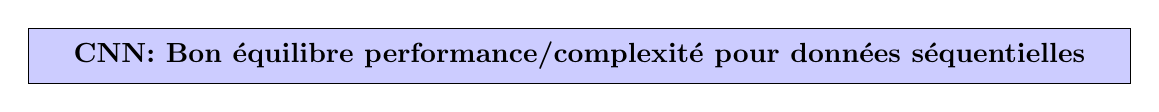
\begin{tikzpicture}
            % Réduction de la hauteur du rectangle (de 1 à 0.7)
            \draw[fill=blue!20] (-2,0) rectangle (12,0.7);
            % Réduction de la police (de \large à \normalsize) et ajustement de la position verticale (de 0.5 à 0.35)
            \node at (5,0.35) {\normalsize\textbf{CNN: Bon équilibre performance/complexité pour données séquentielles}};
        \end{tikzpicture}
    \end{center}
\end{frame}

\begin{frame}{Démonstration Live et Code}
    \begin{block}{Notebook Jupyter Complet}
        \begin{itemize}
            \item \textbf{Disponible}: \url{https://github.com/simoghost99/DeepCAPE-CNN}
            \item \textbf{Structure}:
            \begin{itemize}
                \scriptsize
                \item 1. Chargement données NetCDF
                \item 2. Préprocessing et échantillonnage
                \item 3. Analyse exploratoire (figures présentées)
                \item 4. Définition modèle CNN
                \item 5. Entraînement avec callbacks
                \item 6. Évaluation et visualisation
                \item 7. Analyse feature importance
            \end{itemize}
            \item \textbf{Reproductibilité}: Random seeds fixés
            \item \textbf{Documentation}: Commentaires détaillés
        \end{itemize}
    \end{block}
    
 \end{frame}
\begin{frame}
    \Huge{\centerline{\textbf{Merci pour votre attention!}}}
    
\vspace{10pt}
    \Large{\centerline{\textbf{Questions \& Discussion}}}
    
    \end{frame}
%----------------------------------------------------------------------------------------

\end{document}
